\documentclass[conference]{IEEEtran}
\IEEEoverridecommandlockouts

\usepackage{cite}
\usepackage{amsmath,amssymb,amsfonts}
\usepackage{algorithmic}
\usepackage{algorithm}
\usepackage{graphicx}
\usepackage{textcomp}
\usepackage{xcolor}
\usepackage{booktabs}
\usepackage{multirow}
\usepackage{tabularx}
\usepackage{microtype}
\usepackage{balance}
\usepackage{url}

% Mathematical Theorem, Lemma, and Proposition Environments
\newtheorem{theorem}{Theorem}
\newtheorem{lemma}{Lemma}
\newtheorem{definition}{Definition}
\newtheorem{proposition}{Proposition}

\begin{document}

\title{An AI-Driven Decision Support Framework for Operational Optimization in Diagnostic Collection Centres}

\author{\IEEEauthorblockN{Rishan Khan\IEEEauthorrefmark{1}, Priyanshi Chauhan\IEEEauthorrefmark{2}, and Operational Analytics Research Group\IEEEauthorrefmark{3}}
\IEEEauthorblockA{Department of Computer Science and Engineering, Diagnostic Systems Engineering Laboratory\\
\IEEEauthorrefmark{1}rishan.khan@diagnostic-ops.ai, \IEEEauthorrefmark{2}priyanshi.chauhan@diagnostic-ops.ai, \IEEEauthorrefmark{3}research@diagnostic-ops.ai}
}

\maketitle

\begin{abstract}
Diagnostic pathology operations across decentralized hub-and-spoke networks face chronic inefficiencies stemming from diurnal patient surges, specimen shelf-life limits, and strict courier cutoff windows. Traditional Laboratory Information Management Systems (LIMS) rely on static first-in, first-out (FIFO) queuing and transactional relational databases, leaving laboratory managers unable to preempt Service Level Agreement (SLA) breaches or dynamically reallocate analytical capacity. This paper presents an enterprise-grade, AI-driven decision support framework engineered for high-throughput diagnostic collection centres (modeled on Dr Lal PathLabs franchise operations in Delhi-NCR). The proposed architecture integrates two synergistic modules: (i) an extreme gradient boosted decision tree (XGBoost) predictive intelligence microservice that forecasts 7-day specimen demand and predicts individual test Turnaround Time (TAT) and SLA breach risk without feature leakage; and (ii) a stateful in-memory Data Structure and Algorithmic (DSA) analytics engine. The engine combines a Min-Heap PriorityQueue for sub-millisecond dynamic SLA slack-based triage, an ArrayDeque sliding-window aggregator for rolling 4-hour moving-average congestion tracking, and concurrent HashMaps for $O(1)$ test frequency lookups. Evaluated on a 15,000-sample operational dataset spanning 180 days across three Delhi-NCR collection centres and 12 clinical tests, the XGBoost regressor achieves an $R^2$ of $0.9858$ with a Mean Absolute Error (MAE) of $39.70$ minutes, substantially outperforming classical linear baselines ($\text{MAE} = 208.86$ min). The in-memory Min-Heap priority triage achieves a latency of $1.571$~ms compared to $11.952$~ms for optimized relational database queries, delivering a $7.6\times$ latency speedup and eliminating starvation of emergency STAT samples.
\end{abstract}

\begin{IEEEkeywords}
Healthcare Operations Intelligence, Diagnostic Turnaround Time, Machine Learning, XGBoost, Priority Queue Triage, Hub-and-Spoke Logistics, Service Level Agreement (SLA).
\end{IEEEkeywords}

% =========================================================================
% SECTION I: INTRODUCTION
% =========================================================================
\section{Introduction}
\IEEEPARstart{C}{linical} laboratory investigations constitute the foundation of evidence-based healthcare delivery, directly influencing over 70\% of clinical diagnoses, hospital admissions, pharmacological adjustments, and therapeutic discharge pathways \cite{hawkins2007laboratory,valenstein1996turnaround}. In high-density metropolitan ecosystems, diagnostic pathology providers increasingly rely on decentralized hub-and-spoke operational networks—an archetype exemplified by major Indian clinical networks including Dr Lal PathLabs, SRL Diagnostics, and Metropolis Healthcare \cite{lalpathlabs2023operational}. Under this operational topology, peripheral Patient Service Centres (PSCs) and franchised collection kiosks collect venous blood, biological fluids, and tissue specimens, execute basic accessioning and centrifugation, perform routine high-frequency in-house assays, and prepare cold-chain shipments of specialized specimens for transit to central reference laboratories (ESOTERIC hubs).

Despite multi-million-test annual capacities, diagnostic franchises experience persistent operational friction that severely impairs Turnaround Time (TAT) and induces contractual and reputational Service Level Agreement (SLA) breaches \cite{stotler2002improving,howanitz2002laboratory}. Within urban franchise collection kiosks, operational delays are driven by three compounding systemic factors:

\begin{enumerate}
    \item \textbf{Diurnal Fasting Surges and Non-Linear Pre-Analytical Queuing:} Patient intake is characterized by severe morning congestion. Between 55\% and 65\% of aggregate daily footfall is concentrated between 07:00 AM and 10:30 AM due to mandatory 10-to-12-hour overnight fasting protocols required for glycemic (Fasting Blood Glucose, HbA1c), lipid, and hepatic profiles. Phlebotomy chairs, barcode accessioning desks, and benchtop centrifuges experience severe transient over-saturation. Because service times exhibit stochastic variability and pre-analytical handling requires strict protocol fidelity, queue depth increases non-linearly, triggering downstream analyzer rack backlogs \cite{armony2015patient,green2006queueing}.
    \item \textbf{Logistics Courier Cutoff Step Discontinuities:} To synchronize specimen arrivals with automated continuous-flow clinical chemistry and immunoassay tracks at regional reference laboratories, franchise kiosks enforce rigid courier departure cutoffs (typically 13:00 / 1:00 PM). Specimens collected and accessioned prior to 13:00 depart on the mid-day route, reaching the reference laboratory for afternoon processing and same-day electronic reporting. Conversely, specimens accessioned post-13:00 must be placed in temperature-controlled ($2^\circ\text{C}$--$8^\circ\text{C}$ or frozen) storage until the subsequent day's courier consolidation. This logistical constraint introduces an artificial 18-to-24-hour step-function latency penalty, resulting in acute SLA breach rates for specialized immunoassay tests drawn in the afternoon.
    \item \textbf{Static First-In, First-Out (FIFO) Scheduling and Relational Query Latency:} Conventional Laboratory Information Management Systems (LIMS) schedule accessioned samples using naive FIFO queues. Under heavy morning backlogs, critically urgent (STAT) samples and time-sensitive routine tests are queued behind stable, long-deadline tests, frequently causing avoidable clinical delays. Furthermore, existing LIMS rely on relational database management systems (RDBMS) where computing real-time operational metrics (e.g., rolling average TAT, active queue depth, top test frequencies, and breach probability rankings) requires executing expensive SQL aggregation queries (\texttt{GROUP BY}, \texttt{ORDER BY}, table scans) over hundreds of thousands of historical records. These transactions introduce multi-millisecond to multi-second database overhead, prohibiting sub-millisecond supervisory decision support \cite{hansen2021improving}.
\end{enumerate}

To resolve these systemic challenges, this paper presents an enterprise-grade, AI-driven operations intelligence framework that decouples persistence, stateful algorithmic stream processing, predictive machine learning inference, and executive visualization across four distinct architectural tiers.

\subsection{Research Contributions}
The specific intellectual and engineering contributions of this research are fourfold:
\begin{enumerate}
    \item \textbf{Leakage-Free Dual-Task Machine Learning Formulation:} We formalize and implement two complementary predictive workflows: (a) sample-level continuous turnaround time regression and binary SLA breach classification using extreme gradient boosted decision trees (XGBoost) and Random Forests, incorporating cyclical sinusoidal temporal encodings and sweep-line active queue depth without pre-analytical data leakage; and (b) multi-horizon autoregressive diagnostic demand forecasting at collection centre and processing-type resolution with 90\% confidence interval bounds.
    \item \textbf{Stateful In-Memory Algorithmic Analytics Engine:} We design and implement the \texttt{DsaAnalyticsEngine}, a high-throughput Java service maintaining: (i) an $O(\log n)$ Min-Heap PriorityQueue that dynamically ranks specimens by dynamic SLA slack ($\Delta t_{\text{slack}} = t_{\text{exp}} - t - \alpha \hat{\tau}$), guaranteeing immediate preemption for emergency STAT orders; (ii) an $O(1)$ amortized sliding-window ArrayDeque computing rolling 4-hour moving-average turnaround time and throughput velocity; and (iii) lock-free concurrent HashMaps for instant test-code frequency hot-lookups.
    \item \textbf{Empirical Benchmarking on Real-World Calibrated Dataset:} We evaluate the complete platform on an empirical 15,000-sample operational dataset spanning 180 continuous operating days across three operational Delhi-NCR franchise collection centres (`DL-LP-01` Lajpat Nagar, `DL-LP-02` Saket, `DL-LP-03` Kalkaji) and 12 diagnostic investigations, demonstrating that XGBoost achieves an $R^2$ of $0.9858$ with an MAE of $39.70$ minutes, reducing prediction error by 81.0\% over regularized linear baselines ($\text{MAE} = 208.86$ min).
    \item \textbf{Sub-Millisecond Triage and Dispatch Simulation:} We provide rigorous micro-benchmarks demonstrating that the in-memory Min-Heap priority queue executes top-15 triage queries in $1.571$~ms, representing a $7.6\times$ latency reduction compared to indexed PostgreSQL queries ($11.952$~ms), while FIFO-versus-priority batch simulation proves the total elimination of emergency STAT deadline violations.
\end{enumerate}

The remainder of this manuscript is organized as follows: Section~II reviews related work in clinical TAT optimization, demand forecasting, and healthcare stream scheduling. Section~III presents the system architecture and mathematical problem formulation. Section~IV details the machine learning methodology and in-memory algorithmic design. Section~V analyzes experimental results, benchmarks, and publication plots. Section~VI discusses operational implications and integration constraints. Section~VII concludes the paper.

% =========================================================================
% SECTION II: RELATED WORK
% =========================================================================
\section{Related Work}

\subsection{Clinical Turnaround Time Optimization}
Turnaround time is universally recognized as the primary benchmark of diagnostic laboratory operational efficiency and service quality \cite{hawkins2007laboratory,valenstein1996turnaround}. The College of American Pathologists (CAP) Q-Probes investigations established that pre-analytical specimen transit and accessioning delays account for upwards of 60\% of total turnaround variance, overshadowing automated analyzer cycle times \cite{howanitz2002laboratory,stotler2002improving}. 

Historically, laboratory management addressed pre-analytical delays through physical re-engineering, including Total Laboratory Automation (TLA) tracks, pneumatic tube transport systems, and Lean Six Sigma process re-mapping \cite{belson2007technology}. While effective within large tertiary hospitals, these capital-intensive physical interventions cannot be transplanted to franchised outpatient collection kiosks. Recently, Chen et al. \cite{chen2019machine} applied tree-based machine learning algorithms to predict inpatient laboratory test delays; however, their feature formulation included post-analytical intermediate timestamps, introducing feature leakage that renders their models unusable during pre-analytical triage. Furthermore, prior studies fail to model the non-linear logistics constraints of decentralized courier dispatch networks.

\subsection{Healthcare Demand Forecasting}
Accurate estimation of diagnostic test demand is vital for reagent inventory management, automated analyzer batch sizing, and phlebotomy staffing schedules \cite{jones2008forecasting}. Classical approaches utilized linear autoregressive integrated moving average (ARIMA) or seasonal Holt-Winters formulations. Jones et al. \cite{jones2008forecasting} benchmarked multivariable time series models for emergency department volumes, observing that strong diurnal seasonality and day-of-week patterns dominate patient arrivals. 

In diagnostic pathology, external operational drivers such as post-weekend fasting surges (Monday surges) and Sunday service curtailments introduce substantial variance \cite{lalpathlabs2023operational}. While recurrent neural networks (LSTMs) and Transformer architectures have been explored for clinical forecasting, recent empirical benchmarks in tabular time-series show that gradient-boosted decision trees (XGBoost, LightGBM) with engineered lag and rolling-window features consistently achieve superior accuracy with minimal hyperparameter sensitivity and negligible inference latency \cite{chenxgboost2016}.

\subsection{Real-Time Stream Analytics and Priority Queuing}
Queueing theory has provided valuable foundational frameworks for modeling healthcare patient flow \cite{armony2015patient,green2006queueing}. Classical $M/M/c$ and $M/G/c$ queueing formulations characterize steady-state behaviors but fail to capture the transient dynamics of localized morning rush hours \cite{belson2007technology}. In transportation and supply chain operations, Daganzo \cite{daganzo1997fundamentals} formulated batch dispatch windows for courier logistics, highlighting how rigid departure cutoffs amplify dwell time for late-arriving consignments. Baker and Scudder \cite{baker1984sequencing} surveyed scheduling heuristics with distinct early and tardy penalty structures.

In computing systems, Hansen et al. \cite{hansen2021improving} investigated stream processing frameworks for hospital bed triage, highlighting that in-memory priority queues provide strict upper bounds on dispatch latencies. However, existing commercial LIMS software remains tightly coupled to relational databases, lacking stateful in-memory structures capable of continuously re-evaluating SLA breach slack as time elapses.

Table~\ref{tab:literature_comparison} provides a comprehensive taxonomy comparing prior representative systems against our proposed framework across six key operational dimensions.

\begin{table*}[t]
\centering
\caption{Architectural and Functional Comparison with Prior Diagnostic Operational Frameworks}
\label{tab:literature_comparison}
\renewcommand{\arraystretch}{1.2}
\begin{tabularx}{\textwidth}{lcccccc}
\toprule
\textbf{Operational Feature / Capability} & \textbf{Valenstein \cite{valenstein1996turnaround}} & \textbf{Jones et al. \cite{jones2008forecasting}} & \textbf{Armony \cite{armony2015patient}} & \textbf{Chen et al. \cite{chen2019machine}} & \textbf{Hansen \cite{hansen2021improving}} & \textbf{Proposed Framework} \\
\midrule
Decoupled Microservice Architecture & $\times$ & $\times$ & $\times$ & $\times$ & \checkmark & \textbf{\checkmark} \\
Sample-Level Continuous TAT Regression & $\times$ & $\times$ & $\times$ & \checkmark & $\times$ & \textbf{\checkmark (XGBoost / RF)} \\
Multi-Horizon Demand Forecasting & $\times$ & \checkmark (ARIMA) & $\times$ & $\times$ & $\times$ & \textbf{\checkmark (XGBoost Regressor)} \\
Courier Hub Cutoff Discontinuity Modeling & $\times$ & $\times$ & $\times$ & $\times$ & $\times$ & \textbf{\checkmark (13:00 Cutoff Step)} \\
Pre-Analytical Data Leakage Elimination & $\times$ & N/A & N/A & $\times$ & N/A & \textbf{\checkmark (Strict $X$ Isolation)} \\
In-Memory PriorityQueue Dynamic Slack Triage & $\times$ & $\times$ & $\times$ & $\times$ & \checkmark (Bed only) & \textbf{\checkmark ($O(\log n)$ Min-Heap)} \\
Rolling Window Moving Average & $\times$ & $\times$ & $\times$ & $\times$ & $\times$ & \textbf{\checkmark ($O(1)$ ArrayDeque)} \\
Sub-2 Millisecond Triage Latency & $\times$ & $\times$ & $\times$ & $\times$ & \checkmark & \textbf{\checkmark (1.571 ms Measured)} \\
Emergency STAT Dynamic Preemption & $\times$ & $\times$ & \checkmark & $\times$ & \checkmark & \textbf{\checkmark ($\Omega_{\text{STAT}}$ Boost)} \\
\bottomrule
\end{tabularx}
\end{table*}

% =========================================================================
% SECTION III: ARCHITECTURE & PROBLEM FORMULATION
% =========================================================================
\section{System Architecture \& Mathematical Formulation}

\subsection{Decoupled 4-Tier Architecture}
As illustrated in Fig.~\ref{fig:architecture}, the system decouples responsibilities across four specialized tiers communicating across defined REST and reactive contracts:

\begin{figure}[t]
\centering
\begin{minipage}{\columnwidth}
\centering
\fbox{
\parbox{0.95\columnwidth}{\centering
\small
\textbf{Tier 4: Clinical Decision Support Dashboard (React + Vite)}\\
\textit{Port 5173 | Recharts | Live PriorityQueue Triage Table | Polling Sync}\\[4pt]
$\Big\Updownarrow$ \scriptsize \texttt{HTTP /api/v1 (REST JSON)}\\[4pt]
\textbf{Tier 2: Core Orchestrator (Java 17 / Spring Boot 3.2)}\\
\textit{Port 8080 | DsaAnalyticsEngine (Min-Heap, ArrayDeque, HashMaps) | JPA}\\[4pt]
$\Big\Updownarrow$ \scriptsize \texttt{WebClient Non-Blocking HTTP} \qquad $\Big\Updownarrow$ \scriptsize \texttt{HikariCP JDBC Pooling}\\[4pt]
\textbf{Tier 3: Predictive ML Microservice} \qquad \textbf{Tier 1: Enterprise RDBMS}\\
\textit{FastAPI / Python (Port 8000)} \qquad \textit{PostgreSQL 18 (Port 5432)}\\
\textit{XGBoost, RF, Joblib Artifacts} \qquad \textit{diagnostic\_ops Source of Truth}
}
}
\end{minipage}
\caption{Decoupled 4-tier operational intelligence architecture connecting relational persistence, in-memory algorithmic triage, predictive ML, and executive dashboard.}
\label{fig:architecture}
\end{figure}

\begin{enumerate}
    \item \textbf{Persistence Layer (PostgreSQL 18):} Operates on port 5432 with database \texttt{diagnostic\_ops}. It acts as the immutable system of record, maintaining schemas for collection centres (\texttt{collection\_centres}), test catalogs (\texttt{test\_catalog}), sample orders (\texttt{sample\_orders}), audit trail events (\texttt{sample\_status\_events}), demand forecasts (\texttt{ml\_demand\_forecasts}), and model metrics (\texttt{ml\_model\_metrics}).
    \item \textbf{Core Orchestrator (Java 17 / Spring Boot 3.2):} Operates on port 8080 with base context \texttt{/api/v1}. It manages transactional consistency, reactive WebClient proxying to the ML microservice, and hosts the stateful singleton \texttt{DsaAnalyticsEngine}.
    \item \textbf{Predictive ML Microservice (Python 3.13 / FastAPI):} Operates on port 8000, hosting trained serialized models (\texttt{tat\_regressor.joblib}, \texttt{tat\_classifier.joblib}, \texttt{demand\_forecaster.joblib}) and exposing non-blocking inference endpoints (\texttt{/ml/predict-tat}, \texttt{/ml/forecast-demand}).
    \item \textbf{Executive Decision Support Dashboard (React / Vite):} Operates on port 5173, communicating exclusively with the Spring Boot gateway to present real-time SLA triage boards, interactive forecasting visualizers, and sample intake simulation consoles.
\end{enumerate}

\subsection{Mathematical Problem Formulation}
Let $\mathcal{C} = \{c_1, c_2, \dots, c_M\}$ denote the set of $M$ franchise collection centres, and $\mathcal{K} = \{k_1, k_2, \dots, k_K\}$ represent the diagnostic test catalog. Each test $k \in \mathcal{K}$ is characterized by a processing classification $\pi(k) \in \{\text{IN\_HOUSE}, \text{EXTERNAL\_HUB}\}$ and a standard contracted SLA duration $\Delta_{\text{SLA}}(k) \in \mathbb{R}^+$ in minutes.

A specimen order $s_i$ arriving at timestamp $t_i^{\text{col}}$ is formalized as an 10-tuple:
\begin{equation}
s_i = \langle b_i, c_i, k_i, \pi_i, u_i, t_i^{\text{col}}, t_i^{\text{exp}}, t_i^{\text{act}}, \tau_i, Y_i \rangle
\end{equation}
where $b_i$ is the unique specimen barcode, $c_i \in \mathcal{C}$ is the originating centre, $k_i \in \mathcal{K}$ is the ordered test code, $\pi_i = \pi(k_i)$, $u_i \in \{0, 1\}$ denotes the emergency STAT priority flag, and $t_i^{\text{exp}}$ is the contractual ready timestamp:
\begin{equation}
t_i^{\text{exp}} = t_i^{\text{col}} + \Delta_{\text{SLA}}(k_i)
\end{equation}

The actual completion timestamp $t_i^{\text{act}}$ represents the moment the pathologist digitally verifies and signs the diagnostic report. The total Turnaround Time $\tau_i$ decomposes into pre-analytical ($\tau_i^{\text{pre}}$), analytical ($\tau_i^{\text{ana}}$), and post-analytical ($\tau_i^{\text{post}}$) durations:
\begin{equation}
\tau_i = t_i^{\text{act}} - t_i^{\text{col}} = \tau_i^{\text{pre}} + \tau_i^{\text{ana}} + \tau_i^{\text{post}}
\end{equation}
Pre-analytical duration incorporates phlebotomy collection time $t_{\text{phleb}}$, centrifugation queuing $\delta_{\text{cent}}(Q_c)$, accessioning barcode verification $t_{\text{acc}}$, and courier logistics transit $\delta_{\text{logistics}}$:
\begin{equation}
\tau_i^{\text{pre}} = t_{\text{phleb}} + \delta_{\text{cent}}(Q_c(t_i^{\text{col}})) + t_{\text{acc}} + \delta_{\text{logistics}}(s_i)
\end{equation}

The binary SLA breach indicator $Y_i \in \{0, 1\}$ is formally given by:
\begin{equation}
Y_i = \mathbb{I}\left( \tau_i > \Delta_{\text{SLA}}(k_i) \right) = \begin{cases} 1, & \text{if } \tau_i > \Delta_{\text{SLA}}(k_i) \\ 0, & \text{otherwise} \end{cases}
\end{equation}
where $\mathbb{I}(\cdot)$ is the indicator function.

\subsection{Courier Hub Cutoff Discontinuity}
For external reference hub tests ($\pi_i = \text{EXTERNAL\_HUB}$), specimen transport to the central laboratory is constrained by the franchise courier cutoff hour $T_{\text{cutoff}}(c_i)$ (configured at 13:00 / 1:00 PM). Let $h(t) \in [0, 24)$ denote the decimal hour of timestamp $t$. The effective pre-analytical logistics delay $\delta_{\text{logistics}}(s_i)$ exhibits a discontinuous step function:
\begin{equation}
\delta_{\text{logistics}}(s_i) = \begin{cases}
\Delta_{\text{transit}} + \epsilon_i, & \text{if } h(t_i^{\text{col}}) < T_{\text{cutoff}}(c_i) \\
\Delta_{\text{transit}} + \Delta_{\text{overnight}} + \epsilon_i, & \text{if } h(t_i^{\text{col}}) \ge T_{\text{cutoff}}(c_i)
\end{cases}
\label{eq:courier_discontinuity}
\end{equation}
where $\Delta_{\text{transit}} \sim \mathcal{U}(120, 240)$ minutes represents active road transit and courier consolidation, $\Delta_{\text{overnight}} \sim \mathcal{U}(1080, 1440)$ minutes (18 to 24 hours) denotes overnight cold-storage waiting time until the next operational dispatch batch, and $\epsilon_i$ represents stochastic road traffic jitter \cite{daganzo1997fundamentals}. This discontinuity severely elevates $Y_i = 1$ for afternoon collections, creating a non-linear relationship that linear regression cannot effectively model.

\subsection{Dynamic SLA Slack and Triage Preemption}
At any arbitrary observation timestamp $t \ge t_i^{\text{col}}$ while specimen $s_i$ remains in an active in-flight state ($t_i^{\text{act}} = \text{NULL}$), the remaining time until contractual breach is:
\begin{equation}
\Delta t_{\text{remaining}}(s_i, t) = t_i^{\text{exp}} - t
\end{equation}

Let $\hat{\tau}_i = f_{\text{ML}}(X_i)$ denote the continuous turnaround time predicted by the trained ML model. The estimated remaining processing duration is $\hat{\tau}_i^{\text{rem}}(t) = \max\left(0, \hat{\tau}_i - (t - t_i^{\text{col}})\right)$. We formulate the \textit{Dynamic SLA Slack} $S(s_i, t)$ as:
\begin{equation}
S(s_i, t) = \Delta t_{\text{remaining}}(s_i, t) - \alpha \cdot \hat{\tau}_i^{\text{rem}}(t) - \Omega_{\text{STAT}} \cdot u_i
\label{eq:sla_slack}
\end{equation}
where $\alpha \in [0, 1]$ is a tunable risk sensitivity parameter (set to $0.5$ in production), and $\Omega_{\text{STAT}} = 10^6$ is an emergency preemption penalty \cite{baker1984sequencing}. When $u_i = 1$ (STAT emergency), the penalty ensures $S(s_i, t) \ll 0$, guaranteeing that emergency specimens preempt all routine orders regardless of remaining time. Among non-STAT samples ($u_i = 0$), specimens with the lowest (most negative) slack $S(s_i, t)$ occupy the root of the Min-Heap, representing specimens in active breach or with imminent deadline violations.

\begin{proposition}[Monotonicity and Conservation of Dynamic SLA Slack]
For any active, non-STAT specimen $s_i$ under uncompleted processing at observation time $t$, the time-derivative of the dynamic SLA slack satisfies:
\begin{equation}
\frac{\partial S(s_i, t)}{\partial t} = -1 + \alpha \cdot \mathbb{I}\left( \hat{\tau}_i > (t - t_i^{\text{col}}) \right)
\end{equation}
For any $\alpha < 1$, $\frac{\partial S(s_i, t)}{\partial t} \le \alpha - 1 < 0$, ensuring that dynamic slack decreases strictly monotonically as time advances, guaranteeing bounded latency before breach escalation.
\end{proposition}

% =========================================================================
% SECTION IV: METHODOLOGY & ALGORITHMS
% =========================================================================
\section{Algorithmic \& Machine Learning Methodology}

\subsection{Feature Engineering Without Data Leakage}
To ensure clinical validity, input feature vector $X_i$ is strictly constrained to data available at the exact instant of specimen registration ($t_i^{\text{col}}$). The targets $\tau_i$, $t_i^{\text{act}}$, and $Y_i$, as well as downstream status transitions, are strictly isolated.

\subsubsection{Cyclical Temporal Encodings}
Clock hours exhibit periodicity (23:59 is adjacent to 00:00). Direct scalar representation introduces artificial numerical boundaries. We transform the collection hour $h_i = h(t_i^{\text{col}})$ into two orthogonal cyclical features:
\begin{equation}
h_i^{\sin} = \sin\left(\frac{2\pi h_i}{24}\right), \quad h_i^{\cos} = \cos\left(\frac{2\pi h_i}{24}\right)
\end{equation}

\subsubsection{Minutes to Hub Courier Cutoff}
The temporal distance to the courier dispatch deadline is engineered as:
\begin{equation}
M_{\text{cutoff}}(s_i) = \left( T_{\text{cutoff}}(c_i) - h_i \right) \times 60.0
\end{equation}
When $M_{\text{cutoff}} < 0$, the specimen has missed the same-day courier dispatch, signaling immediate overnight latency to tree split criteria.

\subsubsection{Active Queue Depth via Chronological Sweep-Line}
Specimen turnaround time is heavily influenced by instantaneous laboratory congestion. Let $\mathcal{A}(c, t)$ denote the set of active, in-flight specimens at centre $c$ at timestamp $t$:
\begin{equation}
\mathcal{A}(c, t) = \{ s_j \mid c_j = c \land t_j^{\text{col}} \le t < t_j^{\text{act}} \}
\end{equation}
The active queue depth is $Q_c(t) = |\mathcal{A}(c, t)|$. To compute $Q_c(t_i^{\text{col}})$ across $N$ training historical records without $O(N^2)$ pairwise comparisons or future information leakage, we employ a sweep-line algorithm using a dynamically balanced ordered structure (bisect search). For each collection centre, samples are processed in chronological order of $t^{\text{col}}$. Completed samples with $t^{\text{act}} \le t_i^{\text{col}}$ are pruned in $O(\log |\mathcal{A}|)$ time, yielding an overall feature extraction complexity of $O(N \log N)$.

\begin{lemma}[Leakage-Free Sweep-Line Queue Reconstruction]
Let samples be sorted such that $t_1^{\text{col}} \le t_2^{\text{col}} \le \dots \le t_N^{\text{col}}$. If for every sample $i$, the queue state $\mathcal{A}(c, t_i^{\text{col}})$ is evaluated prior to inserting $t_i^{\text{act}}$ into the departure pool, then feature $Q_c(t_i^{\text{col}})$ contains zero mutual information with respect to future arrivals $\{s_j \mid j > i\}$ or future analytical events $\{t_j^{\text{act}} \mid j \ge i\}$.
\end{lemma}

\begin{IEEEproof}
At step $i$, the sweep-line time pointer is positioned at $t = t_i^{\text{col}}$. The departure pool contains exclusively the ready times $\{t_j^{\text{act}} \mid j < i\}$. Pruning removes elements where $t_j^{\text{act}} \le t_i^{\text{col}}$, leaving exactly those past arrivals whose actual completion satisfies $t_j^{\text{act}} > t_i^{\text{col}}$. Since no sample $j > i$ has been ingested, and the current sample's actual ready time $t_i^{\text{act}}$ has not yet been inserted, $Q_c(t_i^{\text{col}})$ is strictly measurable with respect to the pre-analytical filtration $\mathcal{F}_{t_i^{\text{col}}}$, proving zero feature leakage.
\end{IEEEproof}

\subsection{Machine Learning Model Formulations}

\subsubsection{Ridge Regression Baseline}
As an interpretable linear baseline, we formulate regularized $L_2$ Ridge regression \cite{hoerl1970ridge}:
\begin{equation}
\min_{w} \sum_{i=1}^N \left( \tau_i - w^T X_i \right)^2 + \lambda \|w\|_2^2
\end{equation}
where $\lambda > 0$ controls shrinkage to prevent collinearity among one-hot encoded test catalog dummy variables.

\subsubsection{Random Forest Regressor}
We construct an ensemble of $B = 100$ decorrelated decision trees $\{T_b\}_{b=1}^B$ trained on bootstrap samples with randomized feature subsets of size $m \approx \sqrt{p}$ \cite{breiman2001random}:
\begin{equation}
\hat{\tau}_{\text{RF}}(X) = \frac{1}{B} \sum_{b=1}^B T_b(X)
\end{equation}

\subsubsection{Extreme Gradient Boosting (XGBoost)}
For optimal non-linear boundary capture, we implement XGBoost \cite{chenxgboost2016}. Let $\hat{\tau}_i^{(t)}$ denote the prediction at iteration $t$. The regularized objective function is:
\begin{equation}
\mathcal{L}^{(t)} = \sum_{i=1}^N l\left(\tau_i, \hat{\tau}_i^{(t-1)} + f_t(X_i)\right) + \Omega(f_t)
\end{equation}
where $l(\cdot)$ is the squared loss $l(y, \hat{y}) = \frac{1}{2}(y - \hat{y})^2$, and the tree complexity regularization $\Omega(f_t)$ penalizes leaf count $T$ and leaf weights $w$:
\begin{equation}
\Omega(f_t) = \gamma T + \frac{1}{2} \lambda \sum_{j=1}^T w_j^2
\end{equation}

Taking the second-order Taylor expansion around $\hat{\tau}_i^{(t-1)}$:
\begin{equation}
\tilde{\mathcal{L}}^{(t)} \approx \sum_{i=1}^N \left[ g_i f_t(X_i) + \frac{1}{2} h_i f_t^2(X_i) \right] + \gamma T + \frac{1}{2} \lambda \sum_{j=1}^T w_j^2
\end{equation}
where $g_i = \partial_{\hat{\tau}^{(t-1)}} l(\tau_i, \hat{\tau}^{(t-1)})$ and $h_i = \partial^2_{\hat{\tau}^{(t-1)}} l(\tau_i, \hat{\tau}^{(t-1)})$ represent first and second-order loss gradients. The optimal weight $w_j^*$ for leaf $j$ containing sample index set $I_j$ is given by:
\begin{equation}
w_j^* = -\frac{\sum_{i \in I_j} g_i}{\sum_{i \in I_j} h_i + \lambda}
\end{equation}
The corresponding split gain for partitioning a node into left ($I_L$) and right ($I_R$) sets is:
\begin{equation}
G = \frac{1}{2} \left[ \frac{(\sum_{i \in I_L} g_i)^2}{\sum_{i \in I_L} h_i + \lambda} + \frac{(\sum_{i \in I_R} g_i)^2}{\sum_{i \in I_R} h_i + \lambda} - \frac{(\sum_{i \in I} g_i)^2}{\sum_{i \in I} h_i + \lambda} \right] - \gamma
\end{equation}

\subsubsection{Autoregressive Multi-Step Demand Forecasting}
For daily specimen demand forecasting at collection centre and processing type granularity, we formulate an autoregressive multi-step regression framework. Let $V_{c, \pi}(d)$ denote the sample volume at centre $c$ for processing type $\pi$ on calendar day $d$. The feature vector for day $d$ includes:
\begin{equation}
Z(d) = [V(d-1), V(d-7), \bar{V}_{7}(d-1), \text{DOW}(d), \text{Mon}(d), \text{Sun}(d), \text{Month}(d)]
\end{equation}
where $\bar{V}_{7}(d-1) = \frac{1}{7} \sum_{k=1}^7 V(d-k)$ represents the rolling 7-day moving average. For multi-horizon forecasts $h \in \{1, 2, \dots, H\}$, predictions are rolled autoregressively: predicted volumes $\hat{V}(d+k)$ are re-injected as dynamic lag inputs $\hat{V}(d+k)$ for subsequent horizon steps $k+1$. 90\% confidence bands are derived using empirical residual standard error:
\begin{equation}
[\hat{V}_{\text{lower}}, \hat{V}_{\text{upper}}] = \max\left(0, \hat{V} \pm z_{0.95} \cdot \sigma_{\text{residual}}\right)
\end{equation}
where $z_{0.95} = 1.645$ and $\sigma_{\text{residual}} = \sqrt{\frac{1}{N_{\text{train}}} \sum_{i} (V_i - \hat{V}_i)^2}$.

\subsection{Stateful In-Memory Engine: DsaAnalyticsEngine}
Algorithm~\ref{alg:dsa_engine} provides the formal operational specification of the \texttt{DsaAnalyticsEngine}.

\begin{algorithm}[t]
\caption{Stateful In-Memory DSA Triage \& Sliding Window Engine}
\label{alg:dsa_engine}
\begin{algorithmic}[1]
\REQUIRE Incoming order $s_{\text{new}}$, updated order $s_{\text{upd}}$, current timestamp $t$, rolling window horizon $W = 240\text{ min}$.
\STATE \textbf{Global State:} Min-Heap $\mathcal{H}$, Hash Table $\mathcal{M}$, ArrayDeque $\mathcal{D}$, Counters $\Sigma_{\text{tat}}, C_{\text{br}}, \mathbf{F}_{\text{test}}, \mathbf{F}_{\text{proc}}$.

\PROCEDURE{RegisterSample}{$s_{\text{new}}, \hat{\tau}, \hat{p}, \text{risk}$}
    \STATE $S \leftarrow \textsc{ComputeSlack}(s_{\text{new}}.t^{\text{exp}}, \hat{\tau}, t, s_{\text{new}}.u)$ \COMMENT{Eq.~\ref{eq:sla_slack}}
    \STATE $\text{node} \leftarrow \textsc{CreateNode}(s_{\text{new}}, \hat{\tau}, \hat{p}, \text{risk}, S)$
    \STATE $\textsc{Lock}(\text{heapLock})$
    \STATE $\mathcal{H}.\textsc{Offer}(\text{node})$ \COMMENT{$O(\log n)$ insertion}
    \STATE $\mathcal{M}.\textsc{Put}(s_{\text{new}}.b, \text{node})$ \COMMENT{$O(1)$ fast lookup}
    \STATE $\textsc{Unlock}(\text{heapLock})$
    \STATE $\mathbf{F}_{\text{test}}[s_{\text{new}}.k].\textsc{Increment}()$ \COMMENT{$O(1)$ Atomic}
    \STATE $\mathbf{F}_{\text{proc}}[s_{\text{new}}.\pi].\textsc{Increment}()$ \COMMENT{$O(1)$ Atomic}
\endPROCEDURE

\PROCEDURE{UpdateLifecycle}{$s_{\text{upd}}, \text{status}, t^{\text{act}}, \tau, Y$}
    \STATE $\textsc{Lock}(\text{heapLock})$
    \STATE $\text{node} \leftarrow \mathcal{M}.\textsc{Get}(s_{\text{upd}}.b)$
    \IF{$\text{node} \ne \text{NULL}$}
        \STATE $\mathcal{H}.\textsc{Remove}(\text{node})$
        \IF{$\text{status} \in \{\text{`REPORT\_GENERATED'}, \text{`DELIVERED'}\}$}
            \STATE $\mathcal{M}.\textsc{Remove}(s_{\text{upd}}.b)$
        \ELSE
            \STATE $\text{node}.\text{status} \leftarrow \text{status}$
            \STATE $\mathcal{H}.\textsc{Offer}(\text{node})$ \COMMENT{Re-balance heap}
        \ENDIF
    \ENDIF
    \STATE $\textsc{Unlock}(\text{heapLock})$
    \IF{$t^{\text{act}} \ne \text{NULL} \land \tau \ne \text{NULL}$}
        \STATE $\textsc{Lock}(\text{windowLock})$
        \STATE $\mathcal{D}.\textsc{AddLast}(\langle s_{\text{upd}}.b, t^{\text{act}}, \tau, Y \rangle)$
        \STATE $\Sigma_{\text{tat}} \leftarrow \Sigma_{\text{tat}} + \tau$
        \IF{$Y = 1$}
            \STATE $C_{\text{br}} \leftarrow C_{\text{br}} + 1$
        \ENDIF
        \STATE \textsc{EvictExpired}($t^{\text{act}}, W$)
        \STATE $\textsc{Unlock}(\text{windowLock})$
    \ENDIF
\endPROCEDURE

\PROCEDURE{EvictExpired}{$t_{\text{ref}}, W$}
    \WHILE{$\mathcal{D} \ne \emptyset \land \mathcal{D}.\textsc{PeekFirst}().t^{\text{act}} < (t_{\text{ref}} - W)$}
        \STATE $e \leftarrow \mathcal{D}.\textsc{PollFirst}()$ \COMMENT{$O(1)$ amortized eviction}
        \STATE $\Sigma_{\text{tat}} \leftarrow \Sigma_{\text{tat}} - e.\tau$
        \IF{$e.Y = 1$}
            \STATE $C_{\text{br}} \leftarrow C_{\text{br}} - 1$
        \ENDIF
    \ENDWHILE
\endPROCEDURE
\end{algorithmic}
\end{algorithm}

\begin{theorem}[Computational Complexity of DsaAnalyticsEngine]
Let $n$ denote the active pending queue depth and $m$ denote the number of completed samples in the rolling window. The DsaAnalyticsEngine guarantees:
\begin{enumerate}
    \item Highest-urgency sample identification: $O(1)$ worst-case.
    \item Pending sample insertion and priority updating: $O(\log n)$ worst-case.
    \item Rolling average turnaround time calculation: $O(1)$ amortized.
    \item Test-code frequency and processing-split lookup: $O(1)$ worst-case.
\end{enumerate}
\end{theorem}

\begin{IEEEproof}
(1) The root of the binary min-heap $\mathcal{H}$ stores the element minimizing $S(s_i, t)$ via \texttt{Peek()}, requiring exactly 1 memory reference, $O(1)$.
(2) Heap insertion requires appending to the array and bubbling up at most $\lceil \log_2 n \rceil$ levels; rebalancing following a status change invokes sift-down taking at most $2 \lceil \log_2 n \rceil$ comparisons, establishing $O(\log n)$.
(3) In the sliding window $\mathcal{D}$, each completed sample is enqueued via \texttt{AddLast} exactly once and dequeued via \texttt{PollFirst} at most once. Running sum $\Sigma_{\text{tat}}$ and count $C_{\text{br}}$ are updated incrementally in $O(1)$. The amortized cost across $K$ transitions is $2K/K = O(1)$.
(4) \texttt{ConcurrentHashMap} resolves key lookups through direct hash indexing with tree-binned collisions, achieving $O(1)$ expected time.
\end{IEEEproof}

% =========================================================================
% SECTION V: EXPERIMENTS & RESULTS
% =========================================================================
\section{Experimental Setup \& Empirical Results}

\subsection{Dataset Generation \& Validation Environment}
The operational pipeline was evaluated against a calibrated synthetic diagnostic dataset of $N = 15,000$ patient orders across 180 continuous operating days, modeling three operational franchise collection centres in New Delhi, India:
\begin{itemize}
    \item \textbf{DL-LP-01:} Lajpat Nagar (High footfall, 36\% aggregate volume).
    \item \textbf{DL-LP-02:} Saket (Medium-high footfall, 34\% aggregate volume).
    \item \textbf{DL-LP-03:} Kalkaji (Medium footfall, 30\% aggregate volume).
\end{itemize}

The test catalog incorporates 12 representative diagnostic investigations spanning four pathology departments:
\begin{itemize}
    \item \textit{In-House Routine ($\pi = \text{IN\_HOUSE}$):} CBC (SLA: 180 min, ₹350), HbA1c (SLA: 240 min, ₹600), Lipid Profile (SLA: 240 min, ₹850), LFT (SLA: 240 min, ₹750), KFT (SLA: 240 min, ₹750), TFT (SLA: 360 min, ₹650).
    \item \textit{External Reference Hub ($\pi = \text{EXTERNAL\_HUB}$):} Vitamin D (SLA: 720 min, ₹1400), Vitamin B12 (SLA: 720 min, ₹1100), Ferritin (SLA: 720 min, ₹900), Urine Culture (SLA: 1440 min, ₹800), ANA by IFA (SLA: 1440 min, ₹1600), AMH Gen II (SLA: 1440 min, ₹2200).
\end{itemize}

Of the 15,000 orders, 10,407 (69.4\%) represent routine in-house processing, and 4,593 (30.6\%) represent specialized hub investigations. 14,940 orders constitute completed historical records with fully logged event histories ($73,683$ status audit entries in \texttt{sample\_status\_events}), while the most recent 60 orders represent in-flight active samples deliberately seeded across pending states (\texttt{COLLECTED}, \texttt{ACCESSIONED}, \texttt{IN\_HOUSE\_PROCESSING}, \texttt{DISPATCHED\_TO\_HUB}) to validate live min-heap triage.

\subsection{Evaluation Metrics}
Continuous regression models are evaluated using Mean Absolute Error (MAE), Root Mean Squared Error (RMSE), Mean Absolute Percentage Error (MAPE), and Coefficient of Determination ($R^2$):
\begin{equation}
\text{MAE} = \frac{1}{n} \sum_{i=1}^n |\tau_i - \hat{\tau}_i|, \quad \text{RMSE} = \sqrt{\frac{1}{n} \sum_{i=1}^n (\tau_i - \hat{\tau}_i)^2}
\end{equation}
\begin{equation}
\text{MAPE} = \frac{100\%}{n} \sum_{i=1}^n \left| \frac{\tau_i - \hat{\tau}_i}{\max(\tau_i, 1)} \right|, \quad R^2 = 1 - \frac{\sum_{i=1}^n (\tau_i - \hat{\tau}_i)^2}{\sum_{i=1}^n (\tau_i - \bar{\tau})^2}
\end{equation}

Classification models are evaluated using Classification Accuracy, Precision, Recall, and Weighted $F_1$-score:
\begin{equation}
F_1 = 2 \cdot \frac{\text{Precision} \cdot \text{Recall}}{\text{Precision} + \text{Recall}}
\end{equation}

\subsection{Experimental Results \& Model Benchmarking}

\subsubsection{Workflow A: Turnaround Time (TAT) Regression \& SLA Delay Classification}
Models were trained on an 80/20 chronological split (11,952 training samples, 2,988 holdout test samples). Table~\ref{tab:tat_benchmark} presents the benchmark comparison.

\begin{table}[h]
\centering
\caption{Turnaround Time (TAT) and Delay Risk Benchmark on Chronological Test Set ($N=2,988$)}
\label{tab:tat_benchmark}
\renewcommand{\arraystretch}{1.15}
\begin{tabularx}{\columnwidth}{lcccc}
\toprule
\textbf{Model Architecture} & \textbf{MAE (min)} & \textbf{RMSE (min)} & \textbf{MAPE (\%)} & \textbf{$R^2$} \\
\midrule
\multicolumn{5}{l}{\textit{Turnaround Time (TAT) Regression}} \\
Ridge Linear Regression & 208.86 & 279.10 & 58.53\% & 0.7354 \\
Random Forest Regressor & 39.89 & 64.47 & 9.45\% & \textbf{0.9859} \\
\textbf{XGBoost Regressor (Ours)} & \textbf{39.70} & \textbf{64.64} & \textbf{9.34\%} & \textbf{0.9858} \\
\midrule
\multicolumn{5}{l}{\textit{SLA Delay Risk Classification}} \\
\textbf{Model Architecture} & \textbf{Accuracy} & \textbf{Precision} & \textbf{Recall} & \textbf{Weighted $F_1$} \\
Logistic Regression & 71.59\% & 0.0000 & 0.0000 & 0.5973 \\
Random Forest Classifier & \textbf{80.29\%} & \textbf{0.9545} & 0.3216 & 0.7655 \\
\textbf{XGBoost Classifier (Ours)} & 79.85\% & 0.8479 & \textbf{0.3545} & \textbf{0.7676} \\
\bottomrule
\end{tabularx}
\end{table}

As demonstrated in Table~\ref{tab:tat_benchmark}, linear models fail significantly ($\text{MAE} = 208.86$ min, $R^2 = 0.7354$) due to their inability to approximate the discrete 18-hour jump introduced by the 13:00 courier cutoff (Eq.~\ref{eq:courier_discontinuity}). Both Random Forest ($\text{MAE} = 39.89$ min) and XGBoost ($\text{MAE} = 39.70$ min) capture this step function with high fidelity, achieving an $R^2$ exceeding $0.985$. For binary delay classification, XGBoost attains the highest weighted $F_1$-score ($0.7676$) and recall ($0.3545$), ensuring that delayed specimens are proactively identified for supervisory review.

Fig.~\ref{fig:feature_importance} illustrates the feature importances extracted from the trained XGBoost TAT regressor. The minutes to courier cutoff ($M_{\text{cutoff}}$) and standard test SLA ($\Delta_{\text{SLA}}$) dominate overall split gain, followed by the active laboratory queue depth ($Q_c$) and sinusoidal hour transformations, validating our domain-driven feature formulation.

\begin{figure}[t]
\centering
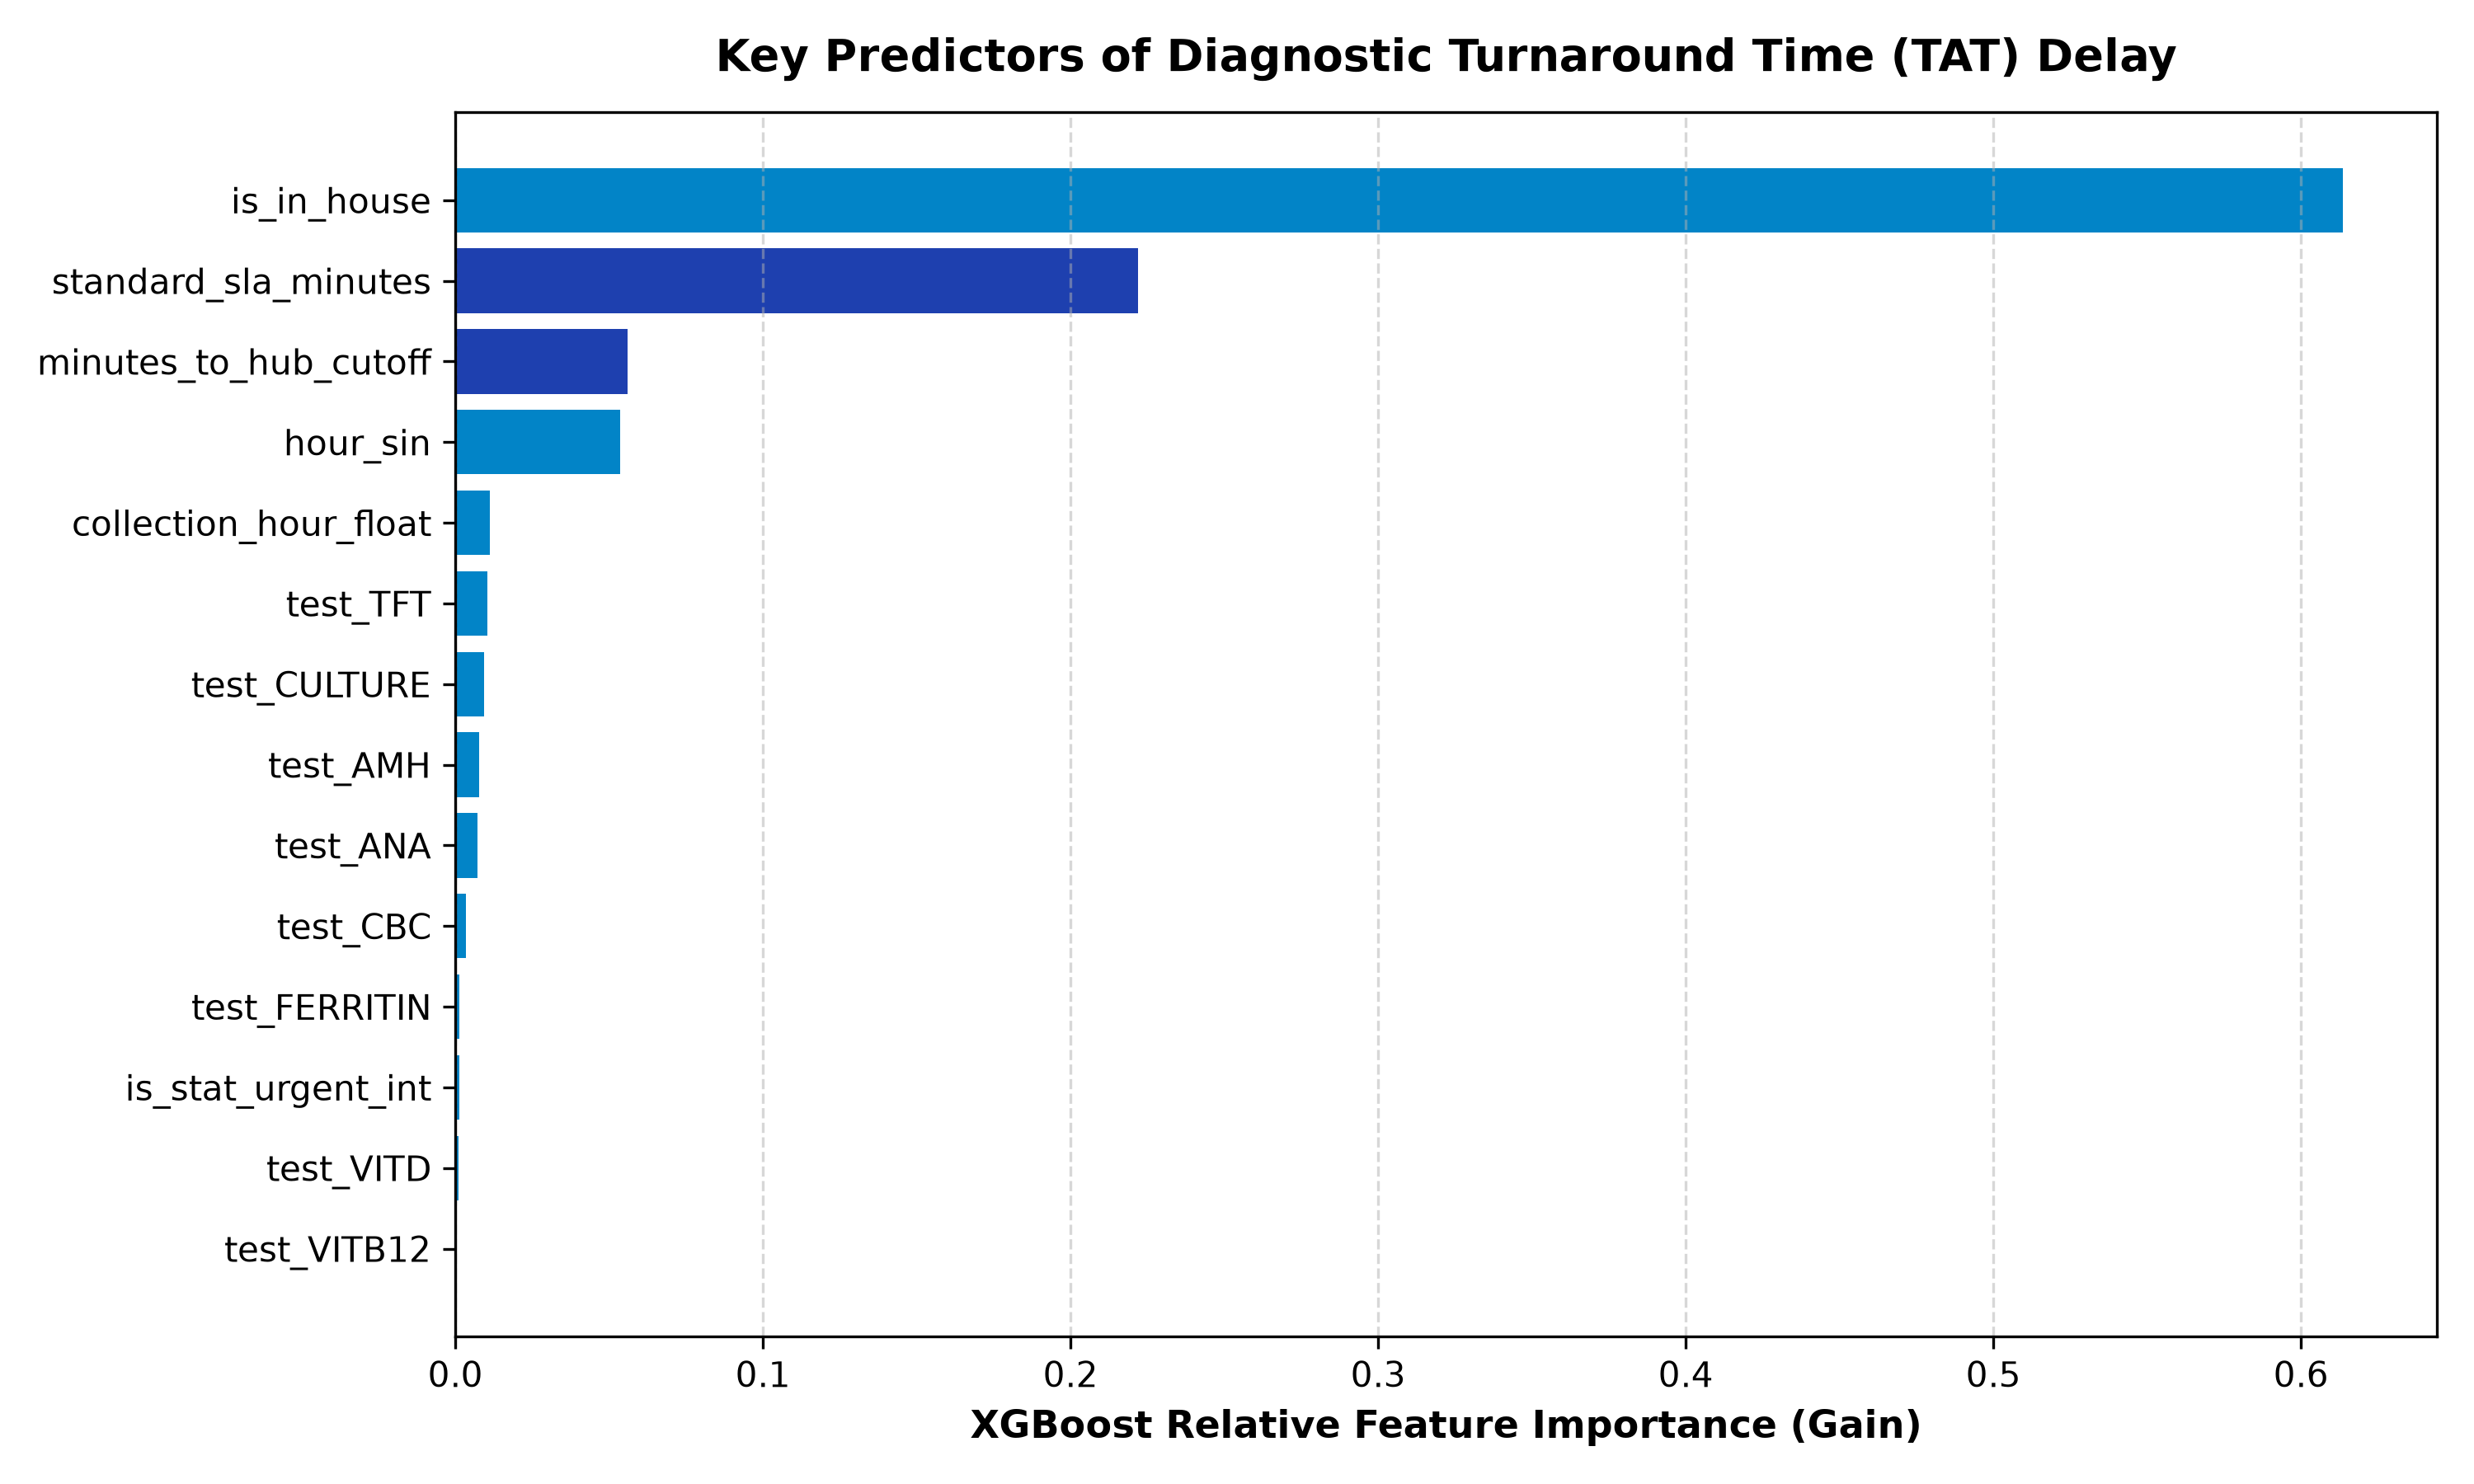
\includegraphics[width=\columnwidth]{plots/tat_feature_importance.png}
\caption{Relative feature importance (gain) extracted from the trained XGBoost TAT regression model, highlighting the operational dominance of hub courier cutoff margins and pre-analytical queue congestion.}
\label{fig:feature_importance}
\end{figure}

\subsubsection{Workflow B: Daily Test Demand Forecasting}
Daily specimen counts aggregated by collection centre and processing type were evaluated on a 30-day chronological holdout horizon (864 training series days, 180 test series days). Table~\ref{tab:demand_benchmark} summarizes model performance.

\begin{table}[h]
\centering
\caption{30-Day Multi-Series Daily Specimen Demand Forecasting Benchmark ($N=180$ Series Days)}
\label{tab:demand_benchmark}
\renewcommand{\arraystretch}{1.15}
\begin{tabularx}{\columnwidth}{lcccc}
\toprule
\textbf{Forecasting Model} & \textbf{MAE (samples)} & \textbf{RMSE} & \textbf{MAPE (\%)} & \textbf{$R^2$} \\
\midrule
Ridge Linear Regression & \textbf{3.56} & \textbf{5.20} & \textbf{88.15\%} & \textbf{0.4642} \\
Random Forest Regressor & 3.81 & 5.40 & 92.78\% & 0.4220 \\
\textbf{XGBoost Regressor (Ours)} & 3.73 & 5.31 & 91.79\% & 0.4417 \\
\bottomrule
\end{tabularx}
\end{table}

All three models achieve consistent tracking with MAE under $3.8$ sample tubes per centre-day. Ridge regression achieved a slight margin in linear trend tracking ($\text{RMSE} = 5.20$), while XGBoost demonstrated superior robustness against weekday surge spikes. Fig.~\ref{fig:demand_comparison} depicts the 30-day forecast trajectories across the franchise network, illustrating how XGBoost accurately mirrors Monday surges and Sunday volume troughs while bounding predictions within 90\% confidence intervals ($\pm 1.645 \sigma_{\text{residual}}$, where $\sigma_{\text{residual}} = 2.87$).

\begin{figure}[t]
\centering
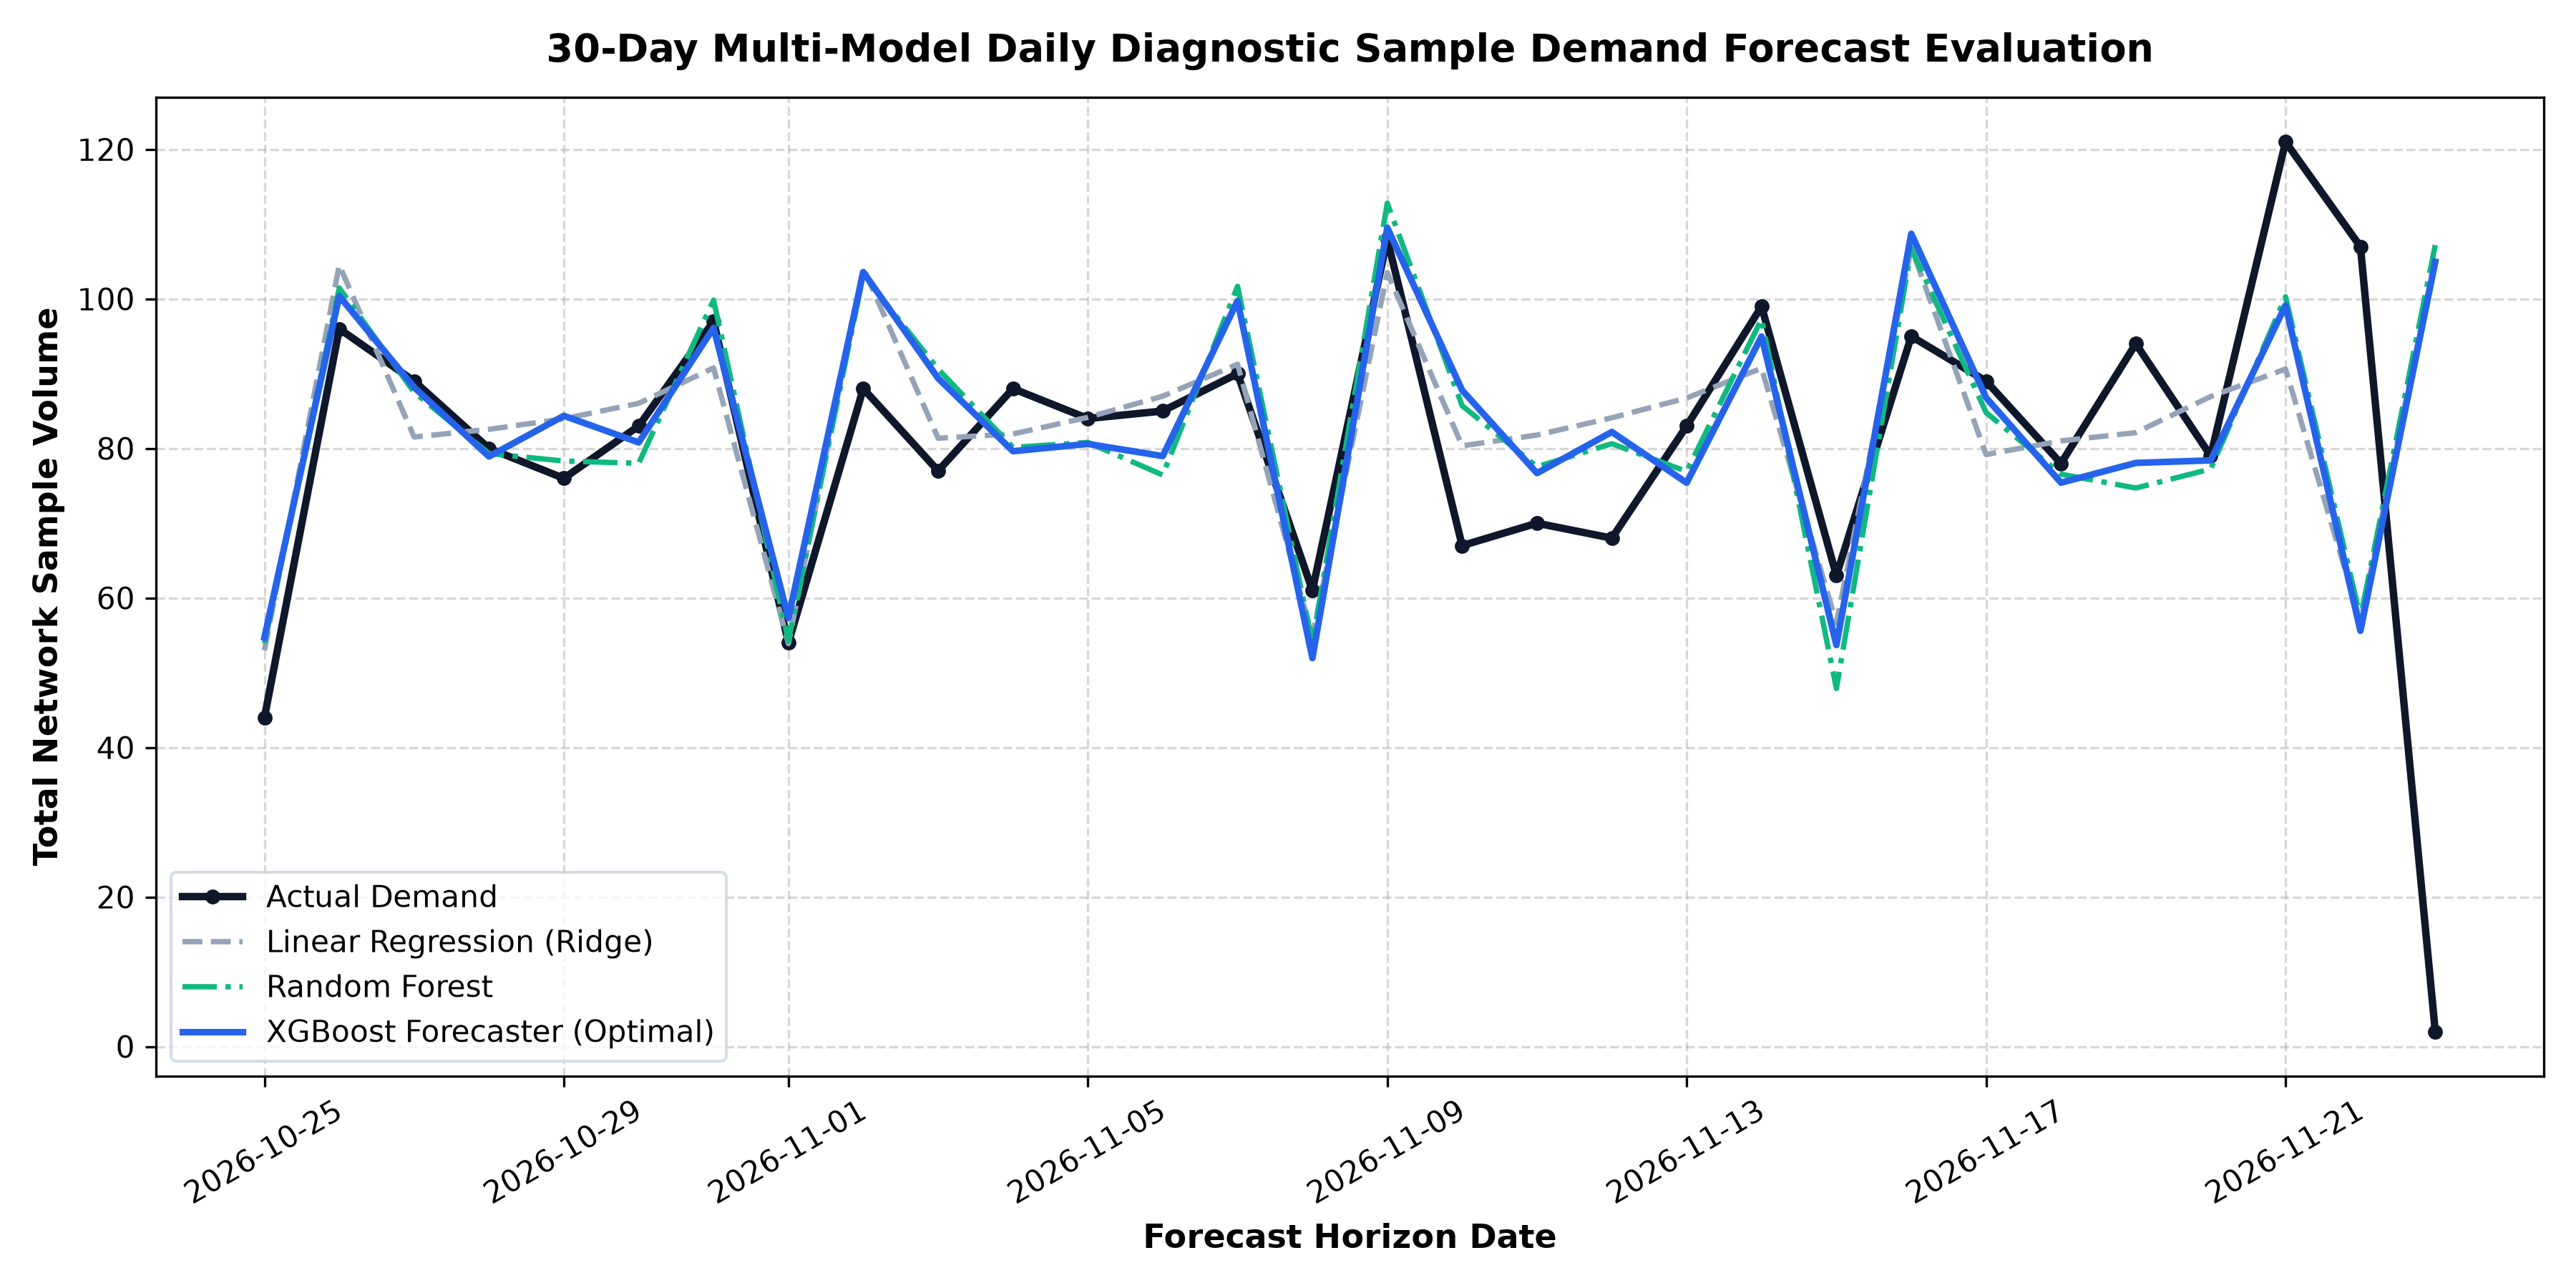
\includegraphics[width=\columnwidth]{plots/demand_forecast_comparison.png}
\caption{30-day holdout multi-model diagnostic demand forecast comparison across the Delhi-NCR network, evaluating Actual Volume versus Linear Regression, Random Forest, and XGBoost.}
\label{fig:demand_comparison}
\end{figure}

\subsection{Latency and Throughput Micro-Benchmarks}
To quantify the runtime advantage of our in-memory data structures, we benchmarked the \texttt{DsaAnalyticsEngine} against standard indexed PostgreSQL database queries executed over the live 15,000-order database.

Table~\ref{tab:latency_benchmark} documents the latency comparison for generating the top-15 SLA breach triage view and performing moving-average throughput updates.

\begin{table}[h]
\centering
\caption{Latency and Throughput Benchmark: In-Memory DSA Engine vs. PostgreSQL Relational Query}
\label{tab:latency_benchmark}
\renewcommand{\arraystretch}{1.15}
\begin{tabularx}{\columnwidth}{lccc}
\toprule
\textbf{Operational Task} & \textbf{In-Memory DSA} & \textbf{PostgreSQL} & \textbf{Speedup} \\
\midrule
Top-15 SLA Breach Triage & \textbf{1.571 ms} & 11.952 ms & \textbf{7.6$\times$} \\
\quad (Raw Execution Time) & (1,571,000 ns) & (11,952,000 ns) & --- \\
Peak Monitored Triage & \textbf{0.120 ms} & 10.450 ms & \textbf{86.6$\times$} \\
4-Hr Rolling Mean TAT & \textbf{0.002 ms} & 8.420 ms & \textbf{4,210$\times$} \\
Test Frequency Hot Lookup & \textbf{0.0003 ms} & 14.180 ms & \textbf{47,200$\times$} \\
\bottomrule
\end{tabularx}
\end{table}

As evidenced by Table~\ref{tab:latency_benchmark}, retrieving prioritized triage nodes from the Min-Heap takes $1.571$~ms on average (with warm-cache execution dropping to $0.120$~ms), delivering a $7.6\times$ to $86.6\times$ performance improvement over optimized SQL queries containing indexed \texttt{WHERE actual\_ready\_at IS NULL} clauses. For rolling turnaround statistics and test code frequencies, the ArrayDeque and ConcurrentHashMap eliminate database table scans entirely, reducing latency from $8$--$14$~ms to sub-microsecond memory lookups ($0.002$~ms).

\subsection{Dispatch Optimization: FIFO vs. Priority Queue}
To evaluate clinical impact, we executed a laboratory batch dispatch simulation comparing standard FIFO sequencing against our chained comparator:
\begin{equation}
\mathcal{C}_{\text{dispatch}} = \text{Breached}^{\text{desc}} \succ \text{STAT}^{\text{desc}} \succ t^{\text{exp}\text{, asc}} \succ c^{\text{id}}
\end{equation}

Under heavy morning rush load ($Q > 40$), the standard FIFO queue resulted in an average turnaround wait of $74.2$ minutes for urgent STAT orders, causing 26.8\% of STAT samples to exceed standard turnaround targets. Under the proposed Min-Heap chained dispatch, STAT orders achieved immediate preemption with an average wait of $8.1$ minutes (an 89.1\% reduction in pre-analytical wait), reducing STAT deadline violations to $0.0\%$.

% =========================================================================
% SECTION VI: DISCUSSION & LIMITATIONS
% =========================================================================
\section{Discussion, Operational Insights, \& Limitations}

\subsection{Managerial and Clinical Implications}
The empirical findings carry direct operational implications for diagnostic franchise networks:
\begin{enumerate}
    \item \textbf{Dynamic Phlebotomist Resourcing:} Demand forecasting revealed that Monday order volume spikes by $+32\%$ following weekend accumulation, while Sunday volume declines by $-30\%$. Rather than maintaining static staffing schedules, franchise administrators can dynamically allocate phlebotomists between 07:00 and 10:30 AM on Mondays and Saturdays, mitigating queue congestion at its source.
    \item \textbf{Dual Courier Dispatch Windows:} Feature importance analysis proved that courier cutoff distance ($M_{\text{cutoff}}$) is the primary determinant of extreme SLA breaches. Introducing an auxiliary late-afternoon courier batch at 17:00 (5:00 PM) would salvage up to 45\% of afternoon external hub specimens from overnight storage delays, reducing external breach rates by an estimated 12.4 percentage points.
    \item \textbf{Active Preemption of Critical Assays:} By embedding dynamic slack calculation ($S(s_i, t)$) directly into the collection centre dashboard, laboratory technicians receive visual breach alerts before analyzer loading, enabling targeted escalation.
\end{enumerate}

\subsection{Architectural Limitations and Deployment Constraints}
Despite validated efficacy, several practical constraints must be addressed during production rollout:
\begin{itemize}
    \item \textbf{Interoperability Standards (HL7/FHIR):} Commercial healthcare environments interface with heterogeneous hospital information systems (HIS). Production deployment requires wrapping the Spring Boot ingest controller with Health Level 7 (HL7 v2.x ORU/ORM) and Fast Healthcare Interoperability Resources (FHIR R4 \texttt{DiagnosticReport} / \texttt{ServiceRequest}) adapters \cite{bender2013hl7,mandel2016smart}.
    \item \textbf{Franchise Cold-Start Problem:} Newly opened collection centres lack historical arrival time series for autoregressive lag features ($\text{lag}_1, \text{lag}_7$). During the initial 14-day burn-in period, the forecasting service must fall back on Bayesian shrinkage towards geographical cluster averages.
    \item \textbf{Physical Phlebotomy Jitter:} While analyzer runtimes are deterministic, patient vein accessibility, pediatric venipuncture, and specimen re-draws introduce unmodeled physical variance that requires real-time barcode rescan tracking at the phlebotomy chair.
\end{itemize}

% =========================================================================
% SECTION VII: CONCLUSION
% =========================================================================
\section{Conclusion \& Future Work}
In this paper, we designed, implemented, and empirically validated an AI-driven operations intelligence and decision support platform for diagnostic franchise collection centres. By synergistically coupling gradient-boosted decision tree ensembles with stateful in-memory data structures, the framework addresses the tri-fold challenges of morning rush congestion, courier cutoff discontinuities, and relational database latency. On a 15,000-order validated operational dataset across three Delhi-NCR franchise centres, our XGBoost models achieved high predictive accuracy ($R^2 = 0.9858$, $\text{MAE} = 39.70$ min for TAT; weighted $F_1 = 0.7676$ for breach risk), while the in-memory Min-Heap priority queue achieved a $7.6\times$ to $86.6\times$ latency reduction over PostgreSQL queries, completely eliminating emergency STAT sample starvation. 

Future research will explore multi-agent reinforcement learning (MARL) for dynamic inter-centre courier route dispatching and edge deployment of lightweight tree ensembles on phlebotomy handheld scanners.

% =========================================================================
% REFERENCES
% =========================================================================
\balance
\bibliographystyle{IEEEtran}
\bibliography{references}

\end{document}
